\documentclass[AMA,Times1COL]{WileyNJDv5} %STIX1COL,STIX2COL,STIXSMALL

\articletype{Article Type}%

\raggedbottom

\begin{document}

\title{GC-EndoGaussian: Residual-Centered Sparse Control for Editable Endoscopic 4D Gaussian Reconstruction}

\author[1]{Anonymous Author(s)}

\authormark{ANONYMOUS}
\titlemark{GC-EndoGaussian: Editable Endoscopic 4D Gaussian Reconstruction}

\address[1]{\orgname{Anonymous Institution}}

\abstract[Abstract]{Dynamic 4D Gaussian Splatting can reconstruct deforming tissue from endoscopic video at high quality and interactive rates, but the learned deformation fields expose no handles for manipulating the reconstruction after training. We study how to add sparse editing handles to a strong endoscopic reconstruction without discarding its captured deformation, and report two findings. First, in a residual-matched comparison the component that preserves fidelity is a dense per-Gaussian residual, not the control-graph architecture: adding the residual to an SC-GS-style sparse-control model improves PSNR from $36.80\pm0.01$ to $37.31\pm0.06$~dB across seeds, halves tracking reprojection error (7.02 to 3.41 pixels), prevents divergence (training collapses on one of four seeds without it), and reduces edit-induced image change leaking outside the edited region from 40\% to 10--12\%. Second, the resulting editable interface can be measured directly: edited tissue follows the commanded handle displacement at a median ratio of 0.96 that is stable across the deforming sequence, the displacement field is identically zero beyond the binding support of the grabbed nodes, and a new edit re-renders in under 5~ms. Our system, GC-EndoGaussian, merges EndoGaussian's dense deformation field with SC-GS-style control nodes under a residual-centered recipe: averaged over four seeds it is 0.11~dB below EndoGaussian on \texttt{pulling\_soft\_tissues} (comparable to seed variation), renders at 205~FPS with 0.07\% extra parameters, and shows no detected tracking difference on SuPer data ($p=0.73$). We edit a learned dynamic reconstruction geometrically at inference time; we do not claim biomechanical simulation.}

\keywords{surgical scene reconstruction, 4D Gaussian Splatting, editable deformation, sparse control nodes, endoscopy}

\maketitle

\renewcommand\thefootnote{}
\footnotetext{\textbf{Abbreviations:} 3DGS, 3D Gaussian Splatting; FPS, frames per second; KNN, K-nearest neighbors; PSNR, peak signal-to-noise ratio; RPE, reprojection error.}

\renewcommand\thefootnote{\fnsymbol{footnote}}
\setcounter{footnote}{1}

\section{Introduction}\label{sec1}

Dense reconstruction of deforming tissue from endoscopic video is an important component of computer-assisted intervention. Neural radiance fields and, more recently, 3D Gaussian Splatting (3DGS)~\cite{kerbl2023gaussian} have improved both visual fidelity and rendering speed, and surgical methods including EndoNeRF~\cite{wang2022endonerf}, EndoGaussian~\cite{liu2024endogaussian}, Deform3DGS~\cite{yang2024deform3dgs}, Endo-4DGS, EndoGS, and SurgicalGaussian reconstruct dynamic endoscopic scenes by learning a canonical representation with a time-dependent deformation field.

These methods \emph{faithfully replay} the observed deformation: the field is a continuous per-Gaussian function with no explicit structure, so after training there is no way to ask ``what would this tissue look like if that flap were displaced here?'' Applications such as interactive visualization, AR re-planning, what-if inspection, and authoring varied tissue configurations for training content need to \emph{control} the reconstruction. We present these as potential applications: our edits are plausible and produced at negligible cost, not biomechanically validated predictions.

Sparse-control methods such as SC-GS~\cite{huang2024scgs} provide a natural editing interface by binding Gaussians to sparse control points and propagating point motion through skinning---but directly replacing a strong endoscopic deformation field with a lower-dimensional sparse-control model can reduce fidelity. The central question of this work is: \emph{how can sparse editing handles be added to an endoscopic 4D Gaussian reconstruction without discarding the deformation already captured by the base model?} Our contributions, in order of importance:

\begin{enumerate}[1.]
\item \textbf{A controlled isolation of the fidelity-preserving component.} In a residual-matched comparison, an SC-GS-style model without a dense per-Gaussian residual loses $0.52$~dB PSNR, roughly doubles tracking error, leaks $40\%$ of edit-induced image change outside the edited region, and collapses on one of four training seeds; the same control architecture with the residual recovers near-baseline reconstruction and tracking, confines edits, and converges on every seed tested. The key component is the residual, not the graph architecture, which we find interchangeable.

\item \textbf{A quantitatively evaluated edit interface for 4D endoscopic Gaussians.} We measure handle-following fidelity ($0.96$ median, stable across the deforming sequence), structurally compact support (zero displacement beyond the binding neighborhood), foldover below $0.5\%$ across magnitudes and timestamps, and sub-5~ms edit-to-render latency. The control-and-skinning paradigm follows prior editable Gaussian work; the contribution is its integration and measurement in a surgical pipeline.

\item \textbf{A residual-centered integration recipe} (translation-only node control, dense position residual, fixed nodes, no coherence regularization) that stays within 0.11~dB of EndoGaussian averaged over four seeds---comparable to seed variation---at 205~FPS with 0.07\% additional parameters.
\end{enumerate}

\section{Related Work}\label{sec2}

\subsection{Dynamic reconstruction and simulation for surgery}

EndoNeRF~\cite{wang2022endonerf} introduced neural rendering for deformable tissue from stereo endoscopic video; 3DGS-based successors~\cite{kerbl2023gaussian} enable much higher rendering rates. EndoGaussian~\cite{liu2024endogaussian} pairs a canonical Gaussian set with a HexPlane-based~\cite{cao2023hexplane} spatio-temporal field and depth supervision. Deform3DGS~\cite{yang2024deform3dgs} uses learnable deformation bases; Endo-4DGS~\cite{huang2024endo4dgs} targets the monocular setting; EndoGS~\cite{zhu2024endogs} and SurgicalGaussian~\cite{xie2024surgicalgaussian} add depth-guided masks and consistency-regularized deformation MLPs; EndoGSLAM~\cite{wang2024endogslam} and Free-SurGS~\cite{guo2024freesurgs} jointly estimate pose; LGS~\cite{liu2024lgs}, HFGS~\cite{zhao2024hfgs}, and EndoSparse~\cite{li2024endosparse} pursue lightweight, high-frequency, and sparse-view variants. None expose sparse handles for post-training manipulation.

A separate line \emph{simulates physics} on endoscopic Gaussian reconstructions. SimEndoGS~\cite{yang2024simendogs} embeds physical properties in reconstructed 3D Gaussians and deforms them with a Material Point Method simulator, and follow-up work~\cite{yang2025sparsesim} accelerates such simulation by driving the scene through sparse control nodes. These methods aim at physically plausible \emph{synthesis} of new deformations from a (quasi-static) reconstruction. GC-EndoGaussian is complementary and makes a deliberately weaker claim: we edit a \emph{learned dynamic} reconstruction geometrically at inference time---the reconstructed motion continues to play back and edits compose with it---without asserting that the response is biomechanically correct. Physics-based simulation could be layered on our control nodes; we evaluate the interface, not tissue mechanics.

\subsection{Editable and sparse-control scene representations}

Beyond surgery, Deformable 3D Gaussians~\cite{yang2024deformable3dgaussians} and 4D Gaussian Splatting~\cite{wu2024fourdgs} extend 3DGS to dynamic scenes with canonical-plus-deformation-field architectures on HexPlane-style~\cite{cao2023hexplane} encodings---the family EndoGaussian adapts. Dynamic 3D Gaussians~\cite{luiten2024dynamic3dgaussians} tracks Gaussians under local-rigidity constraints, GaussianFlow~\cite{gao2024gaussianflow} supervises dynamics with optical flow, and PhysGaussian~\cite{xie2024physgaussian} replaces learning with an MPM simulator. Closest to us, SC-GS~\cite{huang2024scgs} propagates sparse control-point motion to dense Gaussians via KNN skinning for handle-based editing, and CoGS~\cite{yu2024cogs} supports direct real-time manipulation. For implicit fields, EditableNeRF~\cite{zheng2023editablenerf} discovers draggable key points on dynamic NeRFs; NeRF-Editing~\cite{yuan2022nerfediting}, CoNeRF~\cite{kania2022conerf}, Instruct-NeRF2NeRF~\cite{haque2023instructnerf2nerf}, and GaussianEditor~\cite{chen2024gaussianeditor} pursue mesh-proxy, attribute, or semantic editing. The control-and-skinning formulation itself generalizes embedded deformation graphs~\cite{sumner2007embedded} and linear blend skinning~\cite{magnenatthalmann1988jld,lewis2000posespace,sumner2004deformationtransfer}; ARAP-style rigidity priors~\cite{sorkine2007arap} motivate the coherence losses usually paired with sparse control, which our ablations (Section~\ref{sec:residual}) show are unnecessary once a dense residual is present, and dual-quaternion skinning~\cite{kavan2007dualquaternion,kavan2008geometricskinning} motivates restricting rotation when translation-only control suffices.

\section{Method}\label{sec3}

\subsection{Base 4D Gaussian reconstruction}

The scene contains $N\approx30\text{k}$ canonical 3D Gaussians with position $x_i$, rotation, scale, opacity, and spherical-harmonic color. At time $t$, a HexPlane-style~\cite{cao2023hexplane} spatio-temporal field produces a per-Gaussian feature from which small heads predict changes in position, rotation, scale, and opacity. Training is two-stage (coarse static geometry, then fine dynamic deformation), supervised by a tool-masked photometric loss, an inverse-depth loss in binocular mode, and total-variation regularization. This dense model reconstructs well but offers no post-training control handles.

\subsection{Sparse control-node graph}

At the start of the fine stage we initialize $M=1024$--$2048$ control nodes by motion-weighted farthest-point sampling (spatial coverage, weighted toward regions with stronger accumulated deformation). Each Gaussian is bound to its $K=4$ nearest nodes with normalized weights
\begin{equation}\label{eq:weight}
w_{ik}=\frac{\exp\!\left(-\lVert x_i-n_k\rVert^2/\sigma^2\right)}
{\sum_{j\in\mathcal N(i)}\exp\!\left(-\lVert x_i-n_j\rVert^2/\sigma^2\right)},
\end{equation}
where $n_k$ is the canonical position of node $k$ and $\mathcal N(i)$ the node set bound to Gaussian $i$. Bindings are rebuilt when densification changes the Gaussian set; node positions are fixed after initialization.

\begin{figure}[t]
\centering
\includegraphics[width=0.78\columnwidth]{figures/pipeline_horizontal.png}
\caption{GC-EndoGaussian adds a sparse control path to the dense deformation model: node translations are blended and a dense per-Gaussian residual is added. Rotation, scale, and opacity remain under the base field.\label{fig:pipeline}}
\end{figure}

\subsection{Node motion, blending, and edit handle}

For each node $k$ and time $t$, an MLP encodes position and time, $h_k^0=\mathrm{MLP}([\gamma(n_k),\gamma(t)])$ with positional encoding $\gamma$, followed by two EdgeConv-style~\cite{wang2019dgcnn} message-passing layers over a KNN node graph. The general implementation outputs a rigid transformation per node and warps Gaussians by linear blend skinning; this full $SE(3)$ form is used for the SC-GS-style comparisons. In the final configuration the graph predicts \emph{translation only} ($R_k=I$), the output layer is initialized to zero (the control path starts as a no-op), and message passing is not essential: a node-wise MLP performs similarly in the residual-matched ablation, indicating that the dense residual, not the graph aggregator, retains fidelity.

With $r_i(t)$ the dense per-Gaussian residual predicted from the base spatio-temporal feature, the final position is
\begin{equation}\label{eq:final}
p_i(t)=x_i+\sum_{k\in\mathcal N(i)}w_{ik}\,t_k(t)+r_i(t),
\end{equation}
while rotation, scale, and opacity come from the base deformation heads. At inference, a user translation $e_k$ on one or more nodes yields
\begin{equation}\label{eq:edit}
p_i^{\mathrm{edit}}(t)=p_i(t)+\sum_{k\in\mathcal N(i)}w_{ik}\,e_k,
\end{equation}
a local, smoothly weighted edit without retraining (control ratio $\approx$15:1 at 2048 nodes for 30k Gaussians). Non-finite deformation outputs are replaced by unmodified values before rasterization.

\begin{figure}[t]
\centering
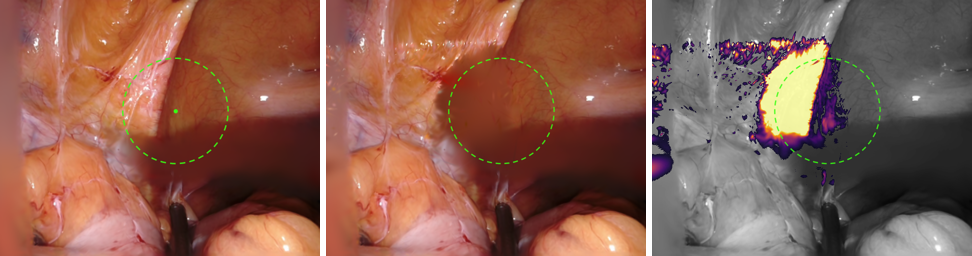
\includegraphics[width=\columnwidth,height=95pt]{figures/edit_reveal_cutting_preview.png}
\caption{Editable tissue retraction on \texttt{cutting\_tissues\_twice}: a local node group (dashed outline) is dragged laterally at inference time, exposing the region behind it without retraining (left: before; middle: after; right: edit magnitude, localized to the retracted region). Controllable visibility only; tissue mechanics are not modeled. The supplementary video shows this retraction ramped, held, and released interactively, and maintained across the deforming sequence.\label{fig:edit_reveal}}
\end{figure}

\subsection{Residual-centered integration recipe}

A sparse graph that replaces the dense field loses reconstruction detail. The final configuration therefore uses: \textbf{(i)} translation-only node control (rotation, scale, opacity stay with the dense model); \textbf{(ii)} a dense per-Gaussian position residual restoring local motion detail a low-dimensional node field cannot represent; \textbf{(iii)} no ARAP, isometric, or temporal coherence losses, which can bias highly non-rigid tissue motion away from the photometric optimum; and \textbf{(iv)} fixed control nodes. Section~\ref{sec:residual} shows the residual is the dominant component; the remaining choices simplify optimization but do not independently explain the fidelity recovery.

\section{Experiments}\label{sec4}

\textbf{Datasets.} Reconstruction is evaluated on the EndoNeRF~\cite{wang2022endonerf} sequences \texttt{pulling\_soft\_tissues} (63 frames) and \texttt{cutting\_tissues\_twice} (156 frames), binocular, $640\times512$, every eighth frame held out. Tracking uses four SuPer~\cite{li2020super} da Vinci trials (26--51 annotated tissue points over 151 frames each), converted via stereo-SGBM depth, tool masks, and static-camera poses; the primary comparison aggregates the four trials, the residual-isolation ablation reports trial 3.

\textbf{Baselines.} \textbf{EndoGaussian} (dense base model, no editing); \textbf{SC-GS-style control} (independent sparse control points, full $SE(3)$ motion, ARAP regularization, adaptive re-seeding, no message passing, 2048 points); \textbf{SC-GS-style + residual} (the same architecture plus our dense residual). All are trained inside the same pipeline to isolate the deformation representation.

\textbf{Metrics and implementation.} PSNR, SSIM, LPIPS, and depth RMSE on held-out frames; tracking as 2D reprojection error with bootstrap 95\% CIs and a paired Wilcoxon test. One NVIDIA H100, PyTorch 2.5.1; 2048 nodes, $K=4$, two graph layers; 1000 coarse + 3000 fine iterations (6000 extended). Seed robustness is mean $\pm$ std over four seeds per configuration (Table~\ref{tab:seeds}). Editing is evaluated with five interface metrics (Section~\ref{sec:edit_eval}): \emph{handle fidelity} (achieved displacement of strongly-bound Gaussians over commanded magnitude), \emph{3D leakage} (normalized displacement beyond twice the handle radius), \emph{pixel leakage} (image change outside the dilated projected footprint of the edited region), \emph{foldover rate} (Gaussian $k$-NN pairs whose relative orientation inverts), and \emph{edit latency} (new edit vector to completed re-render); each aggregates 32 edits (8 handle draws $\times$ 4 magnitudes, 1--8\% of extent, handle radius $0.10\times$ extent), and a temporal sweep repeats the core metrics at five timestamps.

\section{Results}\label{sec5}

\subsection{Reconstruction remains close to the dense baseline}

Under the standard schedule on \texttt{pulling\_soft\_tissues}, the editable model is 0.11~dB lower in PSNR averaged over four seeds (Table~\ref{tab:seeds}); per-configuration seed variation is $\leq 0.09$~dB, so the single-seed gaps in Table~\ref{tab:recon} should be read at that granularity. Under the extended schedule the difference is 0.15~dB (\texttt{pulling}) and 0.13~dB (\texttt{cutting}); SSIM, LPIPS, and depth RMSE remain close but consistently favor the dense baseline. These results show a small, measurable reconstruction cost---not numerical equivalence.

\begin{table*}[t]%
\centering
\caption{Reconstruction under matched optimization schedules. $\Delta$PSNR is GC-EndoGaussian minus EndoGaussian.\label{tab:recon}}%
\begin{tabular*}{\textwidth}{@{\extracolsep\fill}lllccccc@{\extracolsep\fill}}
\toprule
\textbf{Dataset} & \textbf{Fine-stage} & \textbf{Method} & \textbf{PSNR}$\uparrow$ & \textbf{SSIM}$\uparrow$ & \textbf{LPIPS}$\downarrow$ & \textbf{Depth-RMSE}$\downarrow$ & \textbf{$\Delta$PSNR} \\
\midrule
pulling & 3000 & EndoGaussian     & 37.27 & 0.9578 & 0.0609 & 2.906 & --- \\
pulling & 3000 & GC-EndoGaussian  & 37.00 & 0.9559 & 0.0638 & 3.139 & $-0.27$ \\
pulling & 6000 & EndoGaussian     & 37.32 & 0.9578 & 0.0509 & 2.646 & --- \\
pulling & 6000 & GC-EndoGaussian  & 37.17 & 0.9567 & 0.0533 & 2.793 & $-0.15$ \\
cutting & 6000 & EndoGaussian     & 39.42 & 0.9696 & 0.0322 & 1.358 & --- \\
cutting & 6000 & GC-EndoGaussian  & 39.29 & 0.9689 & 0.0339 & 1.384 & $-0.13$ \\
\bottomrule
\end{tabular*}
\end{table*}

\begin{table}[t]%
\centering
\caption{Seed robustness on \texttt{pulling\_soft\_tissues} (standard schedule); mean $\pm$ std over converged seeds. The residual-free model \emph{collapsed on one of four completed seeds} (to 7.5~dB); no residual-equipped configuration failed.\protect\footnotemark\label{tab:seeds}}%
\begin{tabular*}{\columnwidth}{@{\extracolsep\fill}lccc@{\extracolsep\fill}}
\toprule
\textbf{Method} & \textbf{PSNR}$\uparrow$ & \textbf{LPIPS}$\downarrow$ & \textbf{Converged} \\
\midrule
EndoGaussian             & $37.19 \pm 0.09$ & $0.062 \pm 0.001$ & 4/4 \\
SC-GS-style, no residual & $36.80 \pm 0.01$ & $0.090 \pm 0.001$ & 3/4 \\
SC-GS-style + residual   & $37.31 \pm 0.06$ & $0.065 \pm 0.000$ & 4/4 \\
GC-EndoGaussian          & $37.07 \pm 0.06$ & $0.065 \pm 0.001$ & 4/4 \\
\bottomrule
\end{tabular*}
\end{table}
\footnotetext{A further residual-free attempt aborted with a GPU memory-access fault during node-graph training; we exclude it from the divergence statistic as a possible infrastructure rather than optimization failure.}

\subsection{Runtime and parameter overhead}

The sparse control path reduces rendering from 285 to 205~FPS---still well above real-time---and adds 0.07\% deformation parameters (85.29~M to 85.35~M). Applying a new edit vector and re-rendering a $640\times512$ frame takes 4.8~ms (median). Schedules are matched by step count (1000+3000); the added graph work increases per-iteration cost, so step parity is not wall-clock parity.

\subsection{Quantitative edit evaluation}\label{sec:edit_eval}

Table~\ref{tab:edit} measures the editing interface on the three budget-matched models of Table~\ref{tab:residual}. All follow the handle at a median fidelity of $0.96$--$0.97$, with \emph{identically zero} displacement beyond the binding support of the grabbed nodes (Figure~\ref{fig:locality})---locality is a structural property of the compact KNN binding, independent of training. Foldover stays below $0.14\%$ of neighbor pairs in the main sweep, and a new edit re-renders in under 5~ms. The behavior is stable over the deforming sequence (Table~\ref{tab:temporal}): handle fidelity is constant across five timestamps, foldover stays below $0.5\%$, and pixel leakage remains bounded, lowest for GC-EndoGaussian (worst-case $10.6\%$ vs.\ $23.7\%$ without the residual); the supplementary video shows the tissue retraction of Figure~\ref{fig:edit_reveal} performed interactively and maintained across the full deforming sequence.

The models differ sharply in \emph{pixel-space} hygiene: without the dense residual, $40\%$ of edit-induced image change falls outside the edited region's footprint, versus $10$--$12\%$ with it. The residual absorbs appearance detail the sparse graph would otherwise distribute globally, so removing it not only costs fidelity (Table~\ref{tab:residual}) but makes edits visually leak. Decomposing the learned motion shows the node field carries $23$--$31\%$ of deformation energy and the residual $69$--$77\%$: the sparse graph is an \emph{interface} over a predominantly dense motion model.

\begin{table}[t]%
\centering
\caption{Edit-interface metrics on \texttt{pulling\_soft\_tissues} (3000 fine-stage iterations); median over 32 edits. Fid.\ = handle fidelity; L\textsubscript{3D} = displacement beyond $2\times$ handle radius; L\textsubscript{px} = image change outside the edited footprint; Fold = foldover; Lat.\ = edit-to-render latency; R.\,frac.\ = motion energy in the residual.\label{tab:edit}}%
\begin{tabular*}{\columnwidth}{@{\extracolsep\fill}lcccccc@{\extracolsep\fill}}
\toprule
\textbf{Method} & \textbf{Fid.}$\uparrow$ & \textbf{L\textsubscript{3D}}$\downarrow$ & \textbf{L\textsubscript{px}}$\downarrow$ & \textbf{Fold}$\downarrow$ & \textbf{Lat.}$\downarrow$ & \textbf{R.\,frac.} \\
\midrule
SC-GS-style, no residual & 0.97 & 0.0\% & 40.4\% & 0.07\% & 4.5 ms & --- \\
SC-GS-style + residual   & 0.97 & 0.0\% & \phantom{0}9.6\% & 0.08\% & 4.7 ms & 0.69 \\
GC-EndoGaussian          & 0.96 & 0.0\% & 12.3\% & 0.05\% & 4.8 ms & 0.77 \\
\bottomrule
\end{tabular*}
\end{table}

\begin{table}[t]%
\centering
\caption{Temporal stability of the edit interface: the core metrics recomputed at five timestamps spanning the sequence ($t\in\{0.1,0.3,0.5,0.7,0.9\}$, median over 4 handle draws at 4\% edit magnitude); mean (worst) over timestamps.\label{tab:temporal}}%
\begin{tabular*}{\columnwidth}{@{\extracolsep\fill}lccc@{\extracolsep\fill}}
\toprule
\textbf{Method} & \textbf{Fid.}$\uparrow$ & \textbf{L\textsubscript{px}}$\downarrow$ & \textbf{Fold}$\downarrow$ \\
\midrule
SC-GS-style, no residual & 0.98 (0.98) & 16.2\% (23.7\%) & 0.17\% (0.17\%) \\
SC-GS-style + residual   & 0.96 (0.96) & 11.9\% (16.5\%) & 0.18\% (0.20\%) \\
GC-EndoGaussian          & 0.95 (0.95) & \phantom{0}7.4\% (10.6\%) & 0.36\% (0.47\%) \\
\bottomrule
\end{tabular*}
\end{table}

\begin{figure}[t]
\centering
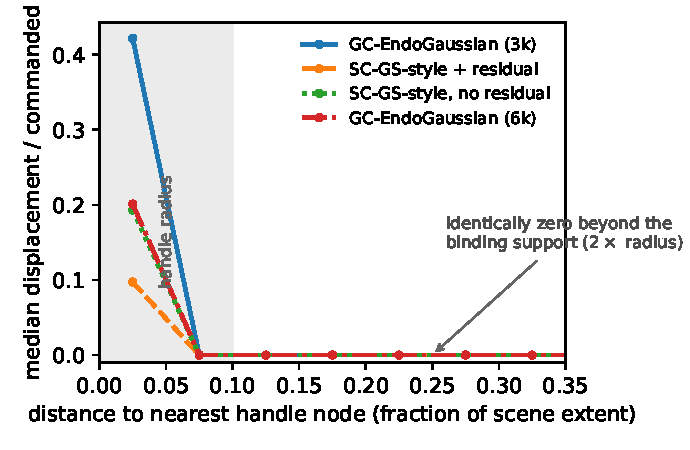
\includegraphics[width=0.6\linewidth]{figures/fig_edit_locality.pdf}
\caption{Edit locality: median per-Gaussian displacement (normalized by commanded magnitude) vs.\ distance to the nearest grabbed node, over 32 edits. Displacement falls off within the handle radius (shaded) and is identically zero beyond the KNN binding support.\label{fig:locality}}
\end{figure}

\textbf{Why the translation-only configuration?} Once the residual is present, the two control architectures are quantitatively close: SC-GS-style + residual attains slightly higher PSNR ($37.31$ vs.\ $37.07$) and lower single-frame pixel leakage ($9.6\%$ vs.\ $12.3\%$), renders at a comparable rate on the same GPU ($216$ vs.\ $206$~FPS), and both converge on all seeds. We keep the translation-only configuration as primary because it has the best tracking ($3.30$ vs.\ $3.41$ pixels on trial 3), the lowest temporal pixel leakage (Table~\ref{tab:temporal}), gives a drag an unambiguous meaning (a pure translation, avoiding the rotation-blending artifacts that motivate dual-quaternion skinning~\cite{kavan2007dualquaternion}), and removes three mechanisms (rotation head, ARAP loss, node re-seeding) with their hyperparameters. SC-GS-style + residual is a validated alternative; both instantiate the same residual-centered recipe, which---not the control architecture---is the load-bearing component.

\subsection{Tracking shows no detected difference from EndoGaussian}

Across the four SuPer trials, median reprojection error is 3.30 pixels for GC-EndoGaussian and 3.47 for EndoGaussian (bootstrap 95\% CIs $[3.14, 3.46]$ and $[3.34, 3.59]$; paired Wilcoxon $p=0.73$). No significant difference is detected; this is not an equivalence test, and with four trials the paired test has minimal power (smallest attainable two-sided $p$ at $n{=}4$ is $0.125$). The residual-free SC-GS-style model provides the informative contrast: on trial 3 its median error is 7.02 pixels, reduced to 3.41 by adding the residual---close to GC-EndoGaussian (3.30) and EndoGaussian (3.47).

\begin{figure*}[t]
\centerline{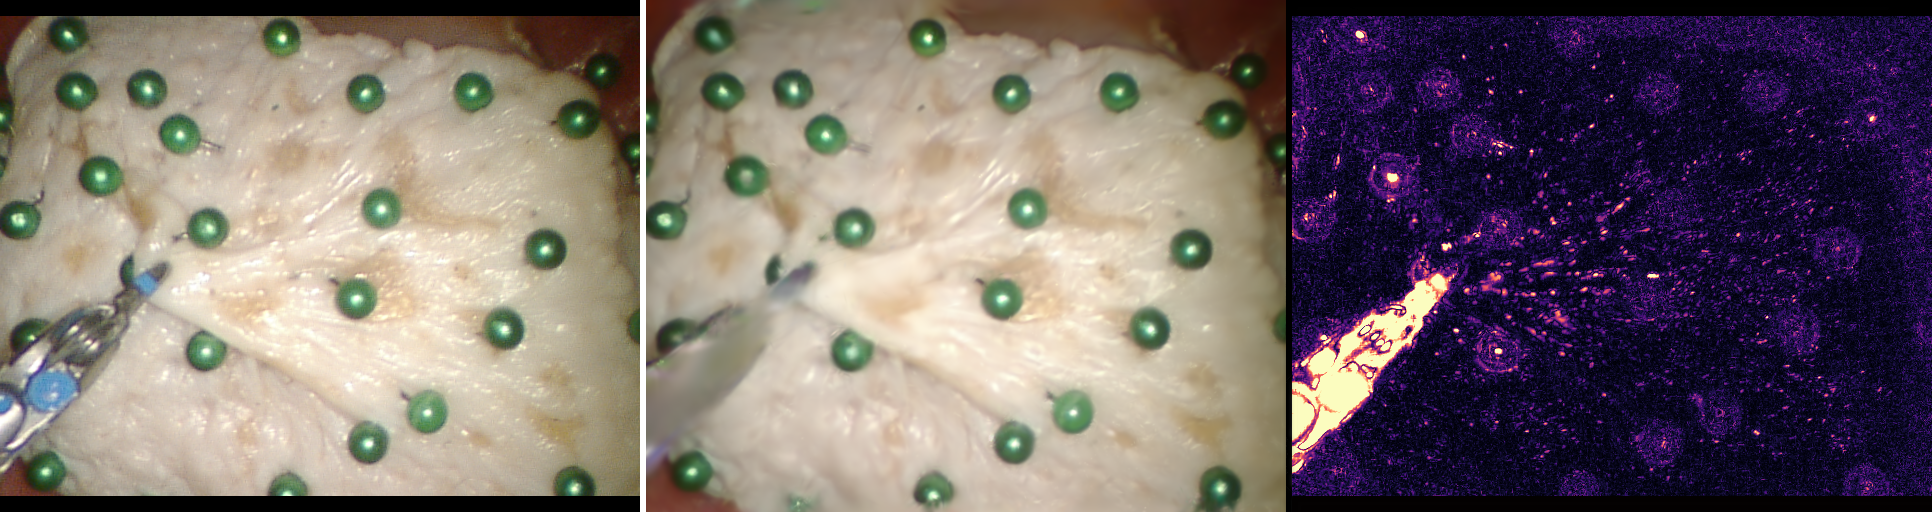
\includegraphics[width=\textwidth,height=9pc]{figures/recon_super_t3_triptych2.png}}
\caption{Reconstruction on SuPer trial 3, frame 90: ground truth, GC-EndoGaussian rendering, and per-pixel error. Discs mark annotated tissue points used in tracking.\label{fig:super}}
\end{figure*}

\subsection{The dense residual is the key fidelity-preserving component}\label{sec:residual}

Which part of the recipe keeps editing reconstruction-neutral---graph message passing, translation-only control, or the residual? Table~\ref{tab:residual}: an SC-GS-style control trained without the residual reaches 36.80~dB and 7.02-pixel tracking error; adding the residual raises PSNR to 37.29~dB and lowers tracking error to 3.41 pixels, recovering the entire gap without adopting our message passing or translation-only control. Across seeds the recovery is $0.52$~dB ($36.80\pm0.01$ to $37.31\pm0.06$; Table~\ref{tab:seeds}), roughly six times the seed variation.

Two observations sharpen this. First, the residual-free model is not merely worse but \emph{less stable}: one of its four completed training runs collapsed, whereas every residual-equipped configuration converged on all four seeds (Table~\ref{tab:seeds}). Second, the gap is visible: Figure~\ref{fig:residual_visual} shows the residual-free model smearing vascular texture and specular highlights that the residual restores. The conclusion is architectural but not graph-specific: a sparse-control editor attached to a high-fidelity endoscopic model should retain a dense per-Gaussian residual. GC-EndoGaussian does not outperform every residual-matched architecture; it is one practical configuration that preserves most of the base fidelity while exposing explicit controls.

\begin{table}[t]%
\centering
\caption{Residual isolation. Reconstruction on \texttt{pulling\_soft\_tissues} after 3000 fine-stage iterations; tracking is median RPE on SuPer trial 3.\label{tab:residual}}%
\begin{tabular*}{\columnwidth}{@{\extracolsep\fill}lcccc@{\extracolsep\fill}}
\toprule
\textbf{Method} & \textbf{PSNR}$\uparrow$ & \textbf{SSIM}$\uparrow$ & \textbf{LPIPS}$\downarrow$ & \textbf{Track RPE}$\downarrow$ \\
\midrule
EndoGaussian, no editing & 37.27 & 0.9578 & 0.0609 & 3.47 \\
SC-GS-style, no residual & 36.80 & 0.9505 & 0.0885 & 7.02 \\
SC-GS-style + residual   & 37.29 & 0.9570 & 0.0649 & 3.41 \\
GC-EndoGaussian          & 37.00 & 0.9559 & 0.0638 & 3.30 \\
\bottomrule
\end{tabular*}
\end{table}

\begin{figure*}[t]
\centering
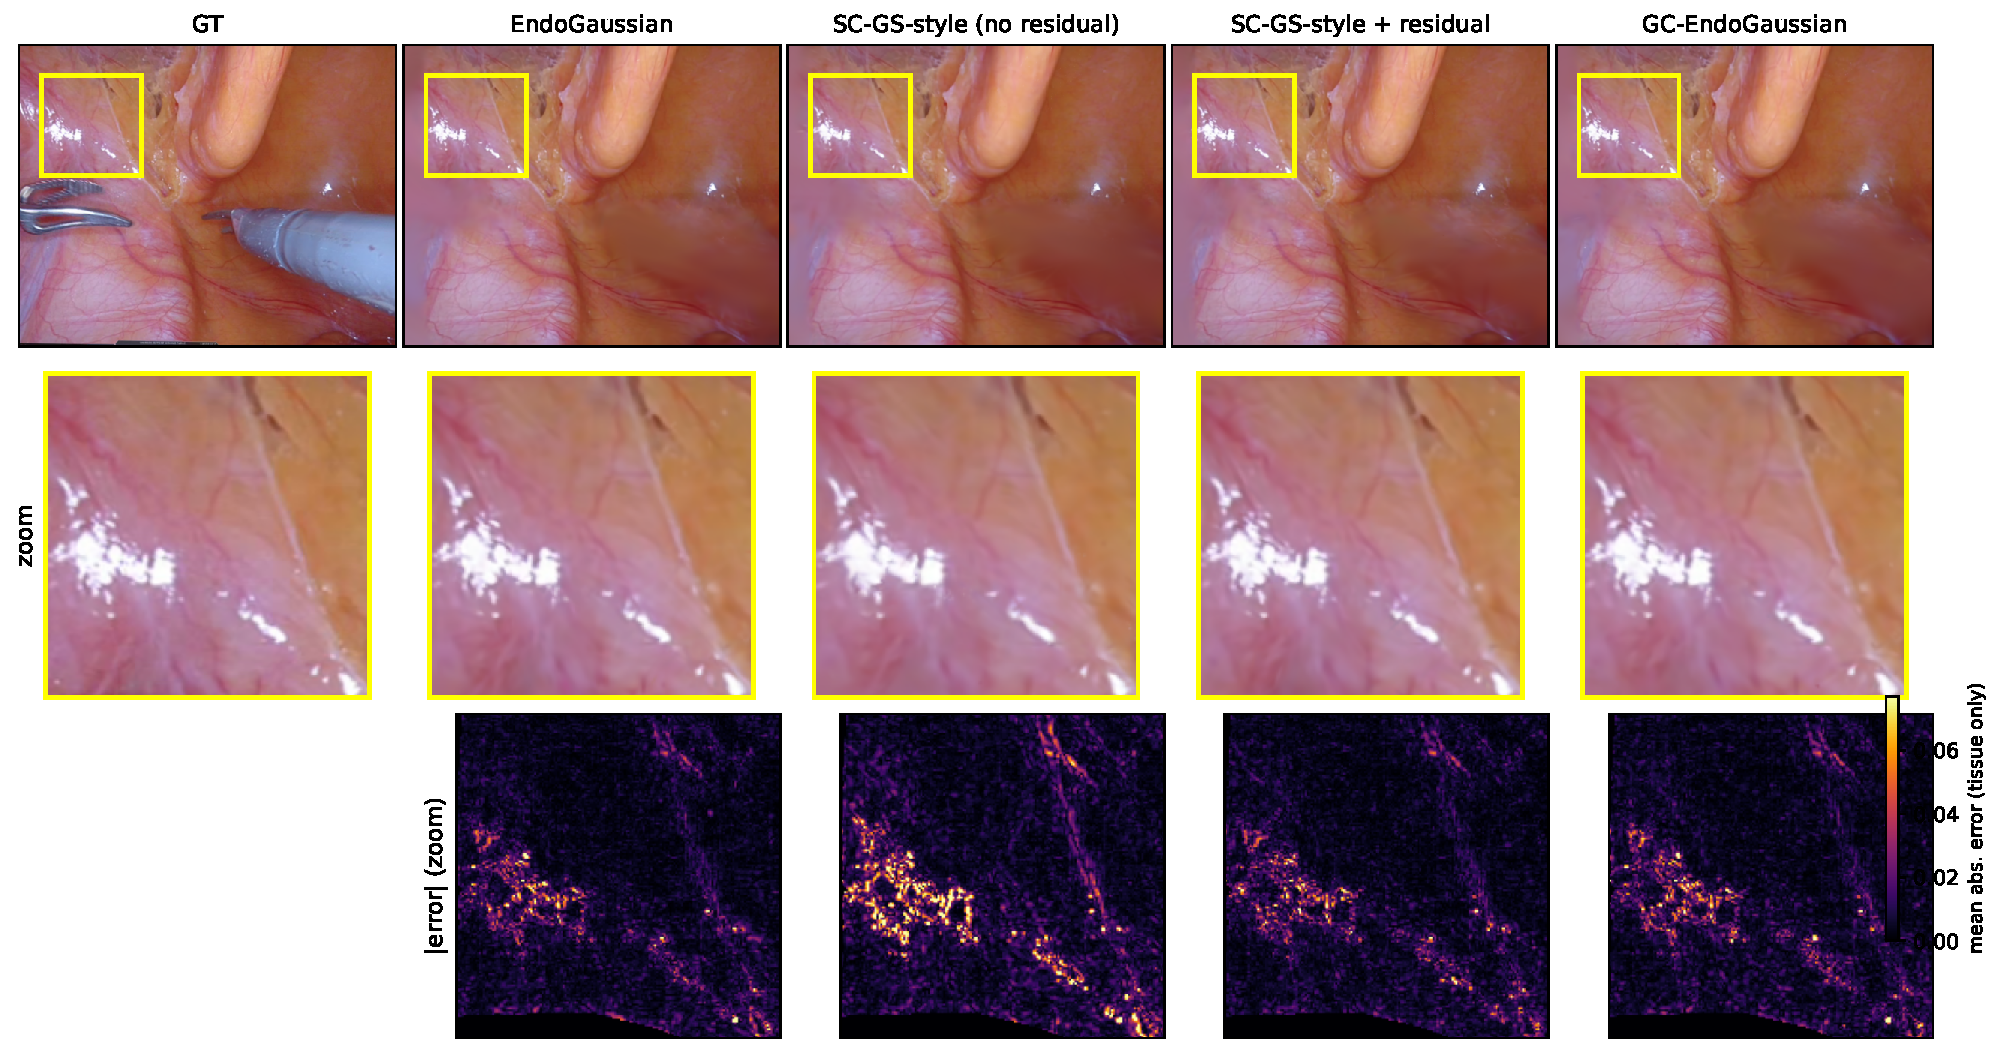
\includegraphics[width=0.8\textwidth]{figures/fig_residual_ablation.pdf}
\caption{What the dense residual fixes (test frame, \texttt{pulling\_soft\_tissues}, matched 3000-iteration budget). Top: rendering with inset location; middle: zoom; bottom: per-pixel error over tissue (tool region excluded; shared scale). The residual-free model (third column) shows visibly higher error on vascular and specular detail; the residual (fourth column) recovers it.\label{fig:residual_visual}}
\end{figure*}

\subsection{Additional ablations and negative results}

Replacing EdgeConv with GAT-style attention changes no conclusion, and removing message passing performs similarly in the residual-matched setting---graph aggregation is not the source of fidelity. The graph also adds little as a reconstruction prior: occlusion-holdout performance matches the dense field, optical-flow supervision does not help (and harms at high weight), and explicit cut modeling does not beat the continuous field at the cut region. The sparse graph contributes an editing interface, not additional reconstruction evidence.

\section{Discussion and Limitations}\label{sec6}

GC-EndoGaussian shows that a sparse editing interface can be added to an endoscopic 4D Gaussian reconstruction while staying close to a strong dense baseline; the dense per-Gaussian residual is necessary for this outcome, for fidelity, edit hygiene, and optimization stability alike. Equally, the results clarify what is not claimed: no reconstruction improvement over EndoGaussian, no tracking equivalence, and no biomechanical simulation---in contrast to physics-embedded approaches~\cite{yang2024simendogs,yang2025sparsesim}, our edits are geometric operations on a learned dynamic reconstruction. Limitations: \textbf{(i)} edits are not biomechanically validated (no material properties, force response, cutting mechanics, or anatomical constraints); \textbf{(ii)} edit evaluation is geometric, not perceptual (no expert user study or comparison to physical simulation); \textbf{(iii)} edits bypass graph message passing, so the graph does not learn to propagate user input according to tissue behavior; \textbf{(iv)} evaluation covers two EndoNeRF scenes and four SuPer trials from one acquisition setting; \textbf{(v)} wall-clock training time and memory remain unmeasured. These position GC-EndoGaussian as an editable visual reconstruction method and a basis for interaction research, not a predictive surgical simulator.

\section{Conclusion}\label{sec7}

We presented a residual-centered study of editable endoscopic 4D Gaussian reconstruction. The main finding is that the dense per-Gaussian residual---not the control-graph architecture---is what preserves fidelity when sparse handles are added: without it, an SC-GS-style model loses 0.52~dB, doubles tracking error, leaks 40\% of edit-induced image change, and collapses on one of four seeds; with it, all four recover. The resulting GC-EndoGaussian interface is measured, not just demonstrated: 0.96 handle fidelity stable across the sequence, structurally compact edit support, foldover below 0.5\%, and sub-5~ms edit-to-render latency, at 205~FPS and 0.11~dB (seed-averaged) from the dense baseline. Future work should quantify perceptual edit plausibility, route edits through learned message passing, and add biomechanical constraints where predictive behavior is required.

\bibliography{wileyNJD-AMA}

\end{document}
